%%%%%%%%%%%%%%%%%%%%%%%%%%%%%%%%%%%%%%%%%
% The Legrand Orange Book
% LaTeX Template
% Version 3.1 (February 18, 2022)
%
% This template originates from:
% https://www.LaTeXTemplates.com
%
% Authors:
% Vel (vel@latextemplates.com)
% Mathias Legrand (legrand.mathias@gmail.com)
%
% License:
% CC BY-NC-SA 4.0 (https://creativecommons.org/licenses/by-nc-sa/4.0/)
%
% Compiling this template:
% This template uses biber for its bibliography and makeindex for its index.
% When you first open the template, compile it from the command line with the 
% commands below to make sure your LaTeX distribution is configured correctly:
%
% 1) pdflatex main
% 2) makeindex main.idx -s indexstyle.ist
% 3) biber main
% 4) pdflatex main x 2
%
% After this, when you wish to update the bibliography/index use the appropriate
% command above and make sure to compile with pdflatex several times 
% afterwards to propagate your changes to the document.
%
%%%%%%%%%%%%%%%%%%%%%%%%%%%%%%%%%%%%%%%%%

%----------------------------------------------------------------------------------------
%	PACKAGES AND OTHER DOCUMENT CONFIGURATIONS
%----------------------------------------------------------------------------------------

\documentclass[
	11pt, % Default font size, select one of 10pt, 11pt or 12pt
	fleqn, % Left align equations
	a4paper, % Paper size, use either 'a4paper' for A4 size or 'letterpaper' for US letter size
	%oneside, % Uncomment for oneside mode, this doesn't start new chapters and parts on odd pages (adding an empty page if required), this mode is more suitable if the book is to be read on a screen instead of printed
]{LegrandOrangeBook}

% Book information for PDF metadata, remove/comment this block if not required 


\addbibresource{sample.bib} % Bibliography file

\definecolor{ocre}{RGB}{243, 102, 25} % Define the color used for highlighting throughout the book

\chapterimage{orange1.jpg} % Chapter heading image
\chapterspaceabove{6.5cm} % Default whitespace from the top of the page to the chapter title on chapter pages
\chapterspacebelow{6.75cm} % Default amount of vertical whitespace from the top margin to the start of the text on chapter pages

%----------------------------------------------------------------------------------------

\begin{document}

%----------------------------------------------------------------------------------------
%	SECTIONING EXAMPLES CHAPTER
%----------------------------------------------------------------------------------------


\part{Production}

%----------------------------------------------------------------------------------------
%	MATHEMATICS EXAMPLES CHAPTER
%----------------------------------------------------------------------------------------

\chapter{Machine de production}

\section{Le début}\index{Theorems}

La machine-outil apparaît au XVe siècle avec les premiers tours destinés au travail du bois.
Leur faible rigidité liée à une structure en bois leur empêche l’usinage d’autres matériaux. Il
faut attendre le XVIIIe siècle pour que des machines-outils en construction métallique apparaissent,
permettant ainsi d’usiner des métaux. On peut citer : le tour à charioter de Vaucanson
en 1751 (voir Figure 1.2-1) et l’ancêtre de la fraiseuse, la machine à raboter de Focq (1761).

\begin{figure}[H] % Use [H] to suppress floating and place the figure/table exactly where it is specified in the text
	\centering % Horizontally center the figure on the page
	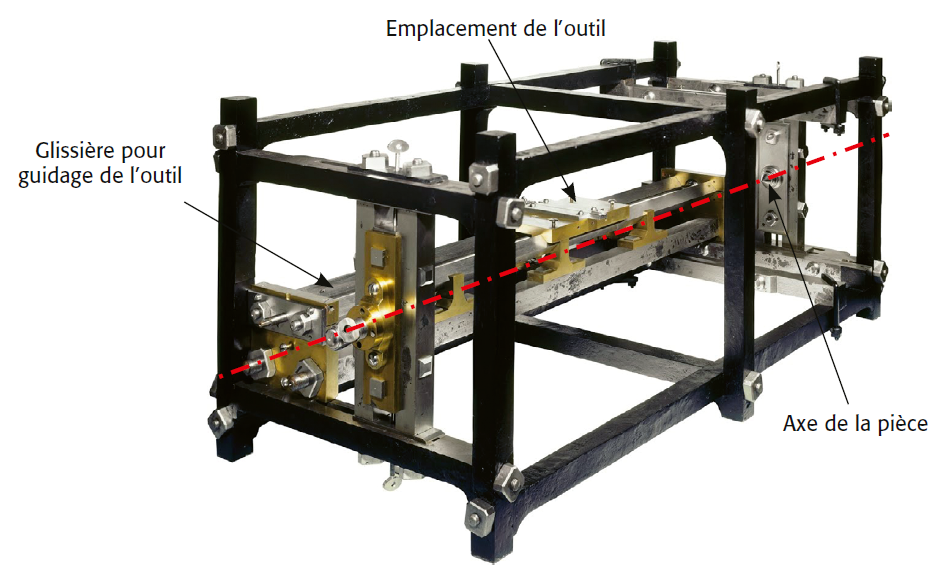
\includegraphics[width=0.8\textwidth]{Images/A01.PNG} % Include the figure image
	\caption{Reproduction du tour de Vaucanson (de 1751)(musée des Arts et Métiers).}
	\label{fig:placeholder} % Unique label used for referencing the figure in-text
\end{figure}


\begin{figure}[H] % Use [H] to suppress floating and place the figure/table exactly where it is specified in the text
	\centering % Horizontally center the figure on the page

	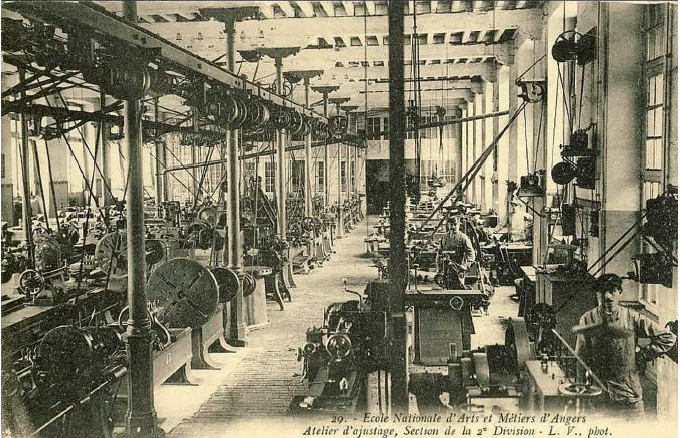
\includegraphics[width=0.8\textwidth]{Images/A02.PNG} % Include the figure image
	\caption{Un atelier typique du début du XXe siècle : vue de l’atelier d’usinage
du campus Arts et Métiers d’Angers (Arts et Métiers).}
	\label{fig:placeholder} % Unique label used for referencing the figure in-text

\end{figure}

En l’espace de trente ans, les vitesses de déplacement des
axes, les vitesses de rotation de broche et donc les vitesses de coupe ont été décuplées. Preuve
des progrès dans les secteurs rattachés à l’usinage : les composants mécaniques comme les
éléments de guidage linéaire ou de guidage en rotation, les composants électrotechniques avec
les directeurs de commande numérique et les chaînes d’asservissement se sont développés. Les
améliorations ne portent pas seulement sur les performances intrinsèques de la machineoutil,
mais aussi sur son environnement. Des systèmes fortement automatisés (palpage laser,
changement outil, lubrification automatique, etc.) se sont largement répandus.


\begin{figure}[H] % Use [H] to suppress floating and place the figure/table exactly where it is specified in the text
	\centering % Horizontally center the figure on the page

	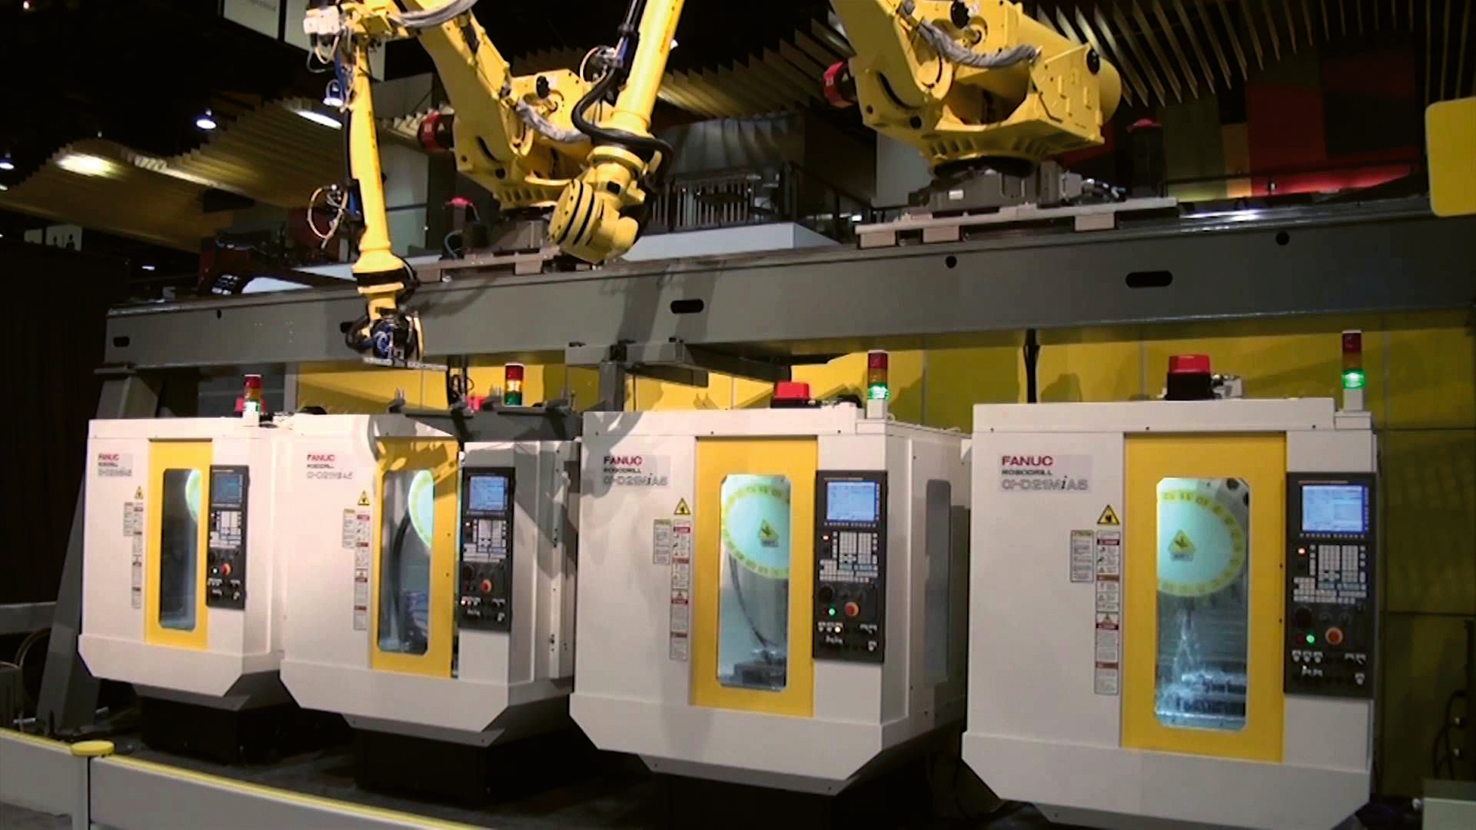
\includegraphics[width=0.8\textwidth]{Images/A03.PNG} % Include the figure image
	\caption{Cellule associant 4 centres d’usinage et 2 robots de chargement-déchargement (Fanuc Robotics).}
	\label{fig:placeholder} % Unique label used for referencing the figure in-text

\end{figure}



\subsection{Combien coûte une machine outil}\index{Theorems!Single Line}

Les données suivantes sont livrées ici à titre indicatif ; les prix indiqués correspondent à une configuration donnée pour un certain fabricant et n’ont d’autre but que de fournir un ordre de grandeur : \\
\begin{itemize}
    \item tour conventionnel ALPHA (dimension entre pointes de 1 000 mm, hauteur de pointe de 200 mm) : 10 000 € en 2016
    \item tour à commande numérique 2 axes HAAS ST35 : 70 000 € en 2018 (sans option)
\end{itemize}

\subsection{Axes des machines outils}

\begin{figure}[H] % Use [H] to suppress floating and place the figure/table exactly where it is specified in the text
	\centering % Horizontally center the figure on the page

	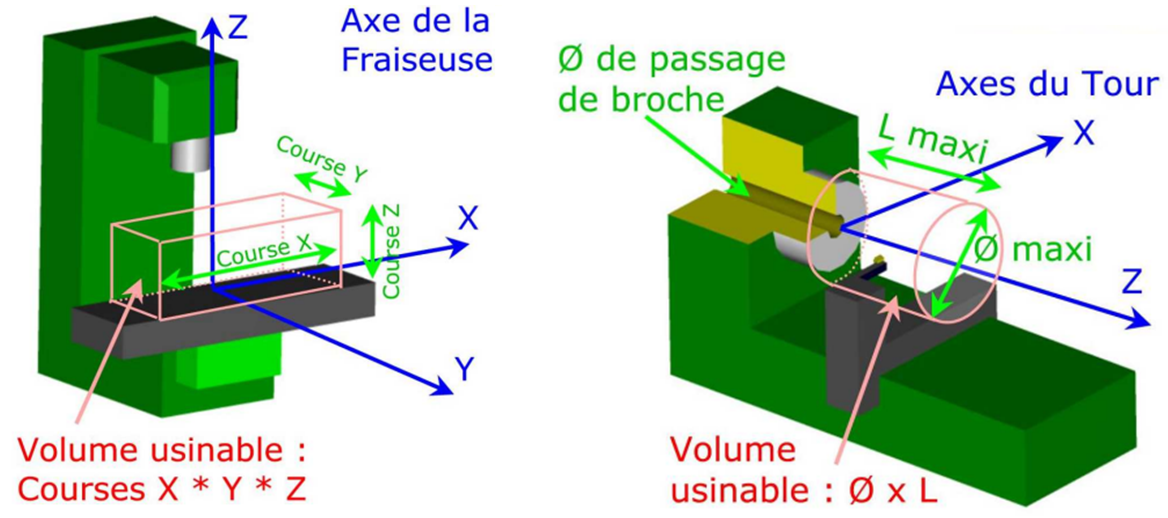
\includegraphics[width=0.8\textwidth]{Images/AA11.PNG} % Include the figure image
	\caption{Axes des MOCN (remarque : L'axe $\Vec{Z}$ est toujours l'axe de la broche)}
	\label{fig:placeholder} % Unique label used for referencing the figure in-text

\end{figure}


Extrait de la norme AFNOR NF Z 60-020 : la présente norme a pour objet de définir une nomenclature des axes et mouvements pour machines à commande numérique en vue de faciliter l’interchangeabilité des données de programmation

\begin{theorem}

    \begin{itemize}
        \item Axe : direction suivant laquelle le mouvement est commandé numériquement en continu en vitesse et position;
        \item L’axe Z : il est situé parallèlement à l’axe de la broche principale quelle que soit la machine ou perpendiculaire à la table pour les machines qui ne possèdent pas de broche;
        \item L’axe X : est associé au mouvement qui défini le plus grand déplacement après avoir situé l’axe Z;
        \item L’axe Y : il forme avec les axes X et Z un trièdre de sens direct. Le sens positif (+) d’un mouvement de chariot provoque l’éloignement de l’outil par rapport à la pièce considérée comme fixe.
    \end{itemize}
\end{theorem}


\subsection{Élément des outils/ porte-outils}

\begin{figure}[H] % Use [H] to suppress floating and place the figure/table exactly where it is specified in the text
	\centering % Horizontally center the figure on the page

	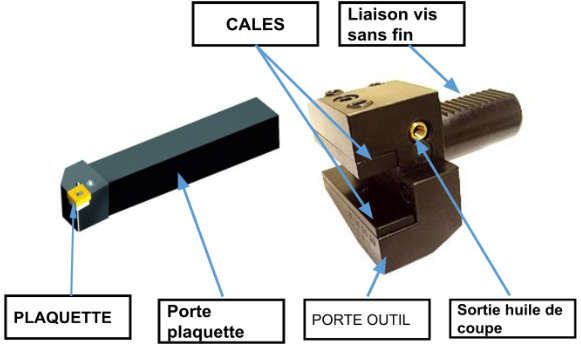
\includegraphics[width=0.85\textwidth]{Images/A5.PNG} % Include the figure image
	\caption{A connaître : Le noms des différents éléments constituant les outils coupants.}
	\label{fig:placeholder} % Unique label used for referencing the figure in-text

\end{figure}


\subsection{Vocabulaire : génération de surfaces}

\begin{figure}[H] % Use [H] to suppress floating and place the figure/table exactly where it is specified in the text
	\centering % Horizontally center the figure on the page

	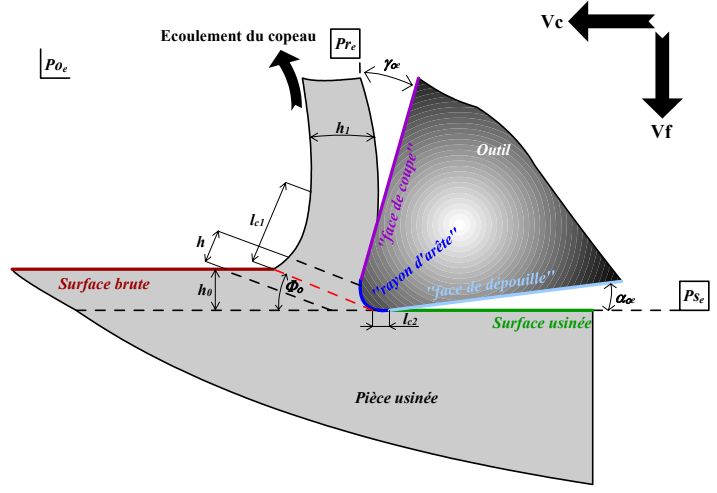
\includegraphics[width=0.85\textwidth]{Images/plaquette1.PNG} % Include the figure image
	\caption{Géométrie locale des contacts copeau-arête élémentaire et arête élémentaire-pièce}
	\label{fig:placeholder} % Unique label used for referencing the figure in-text

\end{figure}


%----------------------------------------------------------------------------------------
%	PRESENTING INFORMATION/RESULTS EXAMPLES CHAPTER
%----------------------------------------------------------------------------------------

\chapterimage{Images/A6.png} % Chapter heading image
\chapterspaceabove{6.25cm} % Whitespace from the top of the page to the chapter title on chapter pages
\chapterspacebelow{7.5cm} % Amount of vertical whitespace from the top margin to the start of the text on chapter pages

%------------------------------------------------

\chapter{Opérations d'usinage}

\section{Opération d'usinage en tournage}\index{Table}
\begin{figure}[H] % Use [H] to suppress floating and place the figure/table exactly where it is specified in the text
	\centering % Horizontally center the figure on the page

	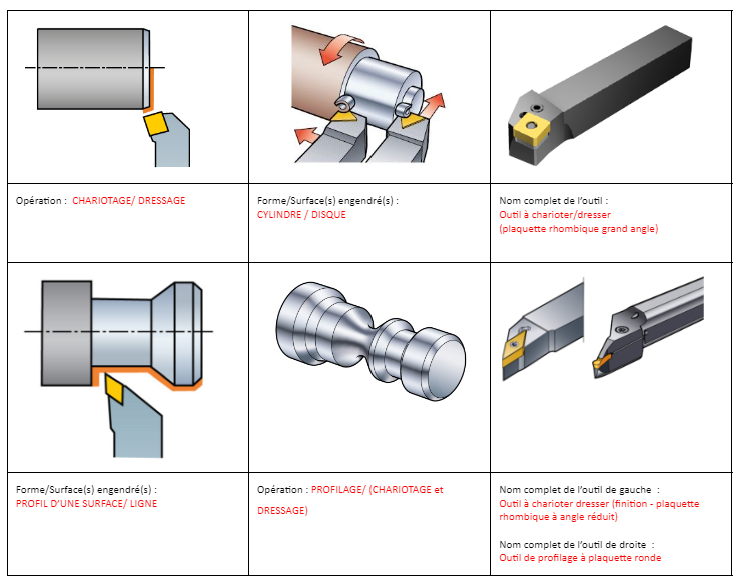
\includegraphics[width=1\textwidth]{Images/CORR21.png} % Include the figure image

	\label{fig:placeholder} % Unique label used for referencing the figure in-text

\end{figure}


\begin{figure}[H] % Use [H] to suppress floating and place the figure/table exactly where it is specified in the text
	\centering % Horizontally center the figure on the page

	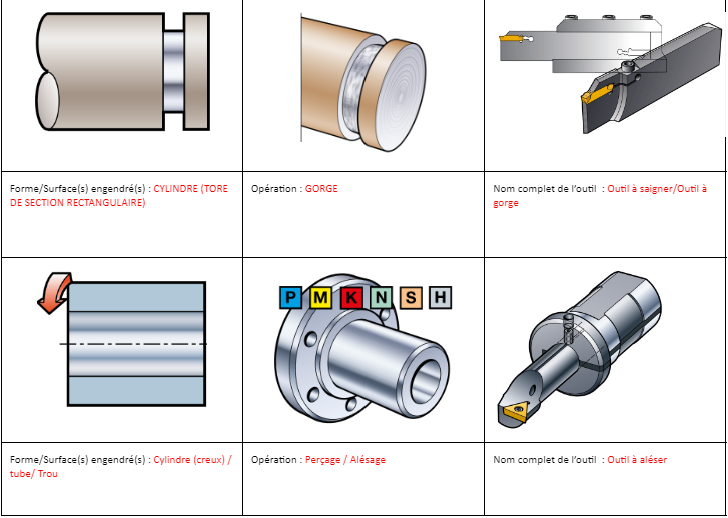
\includegraphics[width=1\textwidth]{Images/CORR22.png} % Include the figure image

	\label{fig:placeholder} % Unique label used for referencing the figure in-text
\end{figure}

\section{Opération d'usinage en fraisage}\index{Figure}


\begin{figure}[H] % Use [H] to suppress floating and place the figure/table exactly where it is specified in the text
	\centering % Horizontally center the figure on the page
	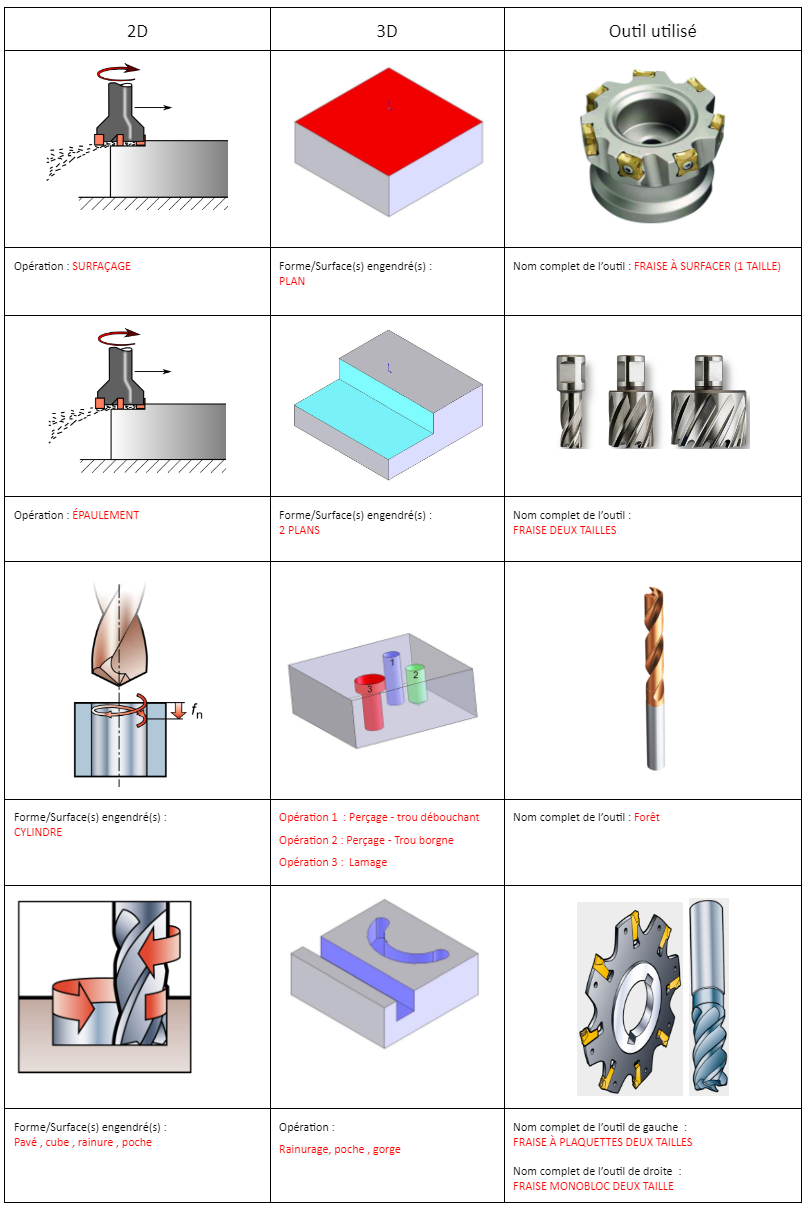
\includegraphics[width=0.85\textwidth]{Images/CORR1.png} % Include the figure image

	\label{fig:placeholder} % Unique label used for referencing the figure in-text
\end{figure}


\subsection{Coupe des éléments coupants}
Les outils ont des formes différentes, plus ou moins complexe, donc plus ou moins onéreux. Pour une entreprise qui cherche à faire des bénéfices, il faudra alors choisir les outils, machines, trajectoires qui nous donne le meilleur compromis " respect du cahier des charges $\rightarrow$ économie " . Aussi, vous pourrez constater que certain outil sont extrêmement proche topologiquement mais n'ont pas exactement les mêmes fonctions ou niveaux de précisions. \\
Le terme "taille" :
\begin{itemize}
    \item Nous parlerons de " Fraise une taille " quand celle-ci aura des arêtes coupantes pour usiner une et une seule surface.
    \item Nous parlerons de "fraise deux taille " quand celle-ci aura des arêtes coupantes d'usiner deux surface.
\end{itemize}

\begin{figure}[H] % Use [H] to suppress floating and place the figure/table exactly where it is specified in the text
	\centering % Horizontally center the figure on the page
	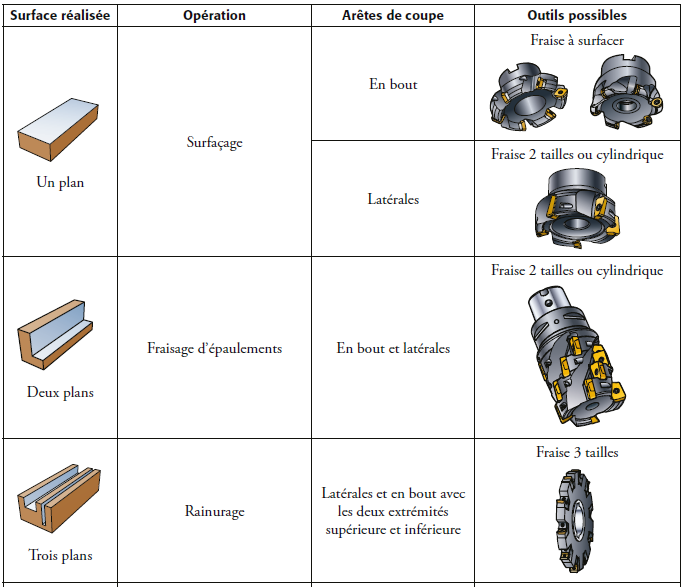
\includegraphics[width=0.85\textwidth]{Images/T12.png} % Include the figure image

	\label{fig:placeholder} % Unique label used for referencing the figure in-text
\end{figure}


\section{Éléments de serrage}
Pour le fraisage et le tournage le serrage à pour but de maintenir la pièce dans la même position tout le long de l'usinage. Pour le tournage cependant il faut en plus que le serrage soit exactement confondu avec l'axe de la broche. En générale nous utiliserons des mors. Vous devez connaître la différences entre des mors durs et mors doux. Pour rappel, un mandrin est constitué de trois mors, qui peuvent être doux ou durs.
\begin{figure}[H] % Use [H] to suppress floating and place the figure/table exactly where it is specified in the text
	\centering % Horizontally center the figure on the page
	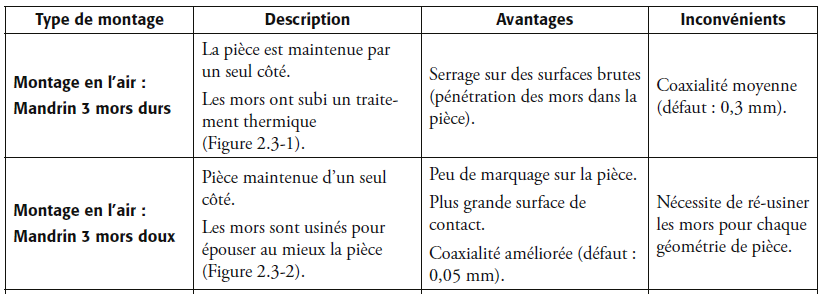
\includegraphics[width=0.85\textwidth]{Images/M1.png} % Include the figure image

	\label{fig:placeholder} % Unique label used for referencing the figure in-text
\end{figure}

Les mors durs sont en contact ponctuel avec la pièce à usiner. Nous aurons donc 3 contacts ponctuels cylindrique. Mécaniquement le contact serait "pivot glissant", mais le serrage nous permet de considérer le contact comme encastrement.
\begin{figure}[H] % Use [H] to suppress floating and place the figure/table exactly where it is specified in the text
	\centering % Horizontally center the figure on the page
	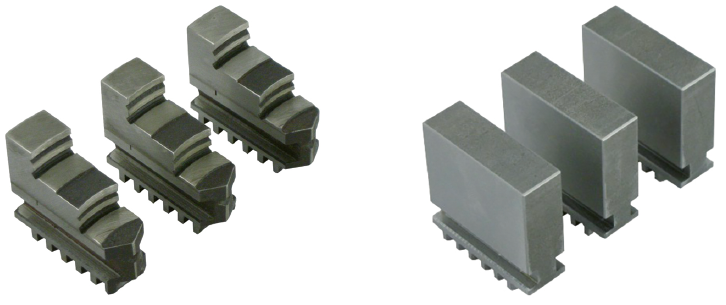
\includegraphics[width=0.85\textwidth]{Images/M2.png} % Include the figure image
    \caption{A gauche, des mors durs, qui constitueront les 3 contacts ponctuels. A droite, trois mors "doux" vendu non usinés, qui devront être usinés au diamètre de la pièce voulue.}

	\label{fig:placeholder} % Unique label used for referencing the figure in-text
\end{figure}

\section{Matière et matériaux}
Pour l'usinage par enlèvement de matière, li faut bien faire la différence entre la matière de la pièce et la matière de l'outil coupant. Nous choisirons la matière de l'outil coupant en fonction de la matière a usiner. L'outil coupant doit évidement toujours être plus "dur" que la matière à usiner.
\begin{figure}[H] % Use [H] to suppress floating and place the figure/table exactly where it is specified in the text
	\centering % Horizontally center the figure on the page
	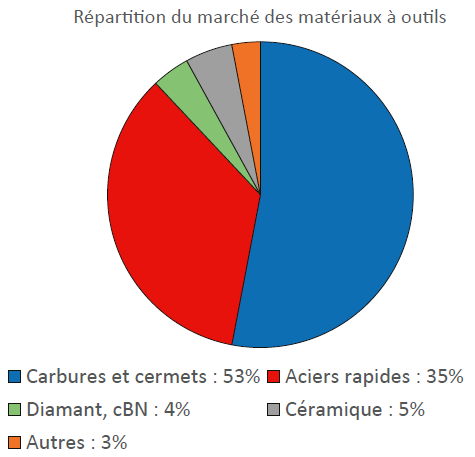
\includegraphics[width=0.6\textwidth]{Images/O1.png} % Include the figure image
    \caption{Matériaux des outils coupant les plus utilisés.}

	\label{fig:placeholder} % Unique label used for referencing the figure in-text
\end{figure}

Les matériaux ci-dessus doivent être choisi en fonction de la pièce à usiner. Beaucoup de tableaux présents dans vos cours ou sur internet vous aiderons à trouver quels matériaux de coupe peuvent correspondre pour usiner une pièce.
\begin{figure}[H] % Use [H] to suppress floating and place the figure/table exactly where it is specified in the text
	\centering % Horizontally center the figure on the page
	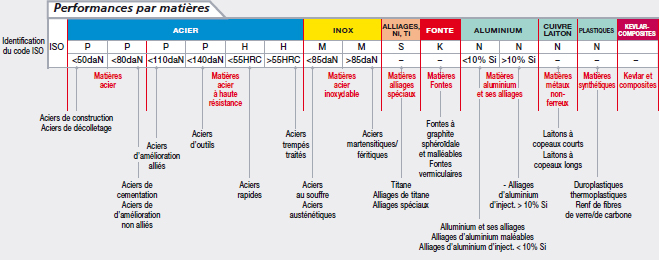
\includegraphics[width=1\textwidth]{Images/O2.jpg} % Include the figure image
    \caption{Exemple de matériaux de pièce à usiner. On regarde le matériaux de la pièce, puis on choisi le matériaux de l'outil coupant.}

	\label{fig:placeholder} % Unique label used for referencing the figure in-text
\end{figure}

%----------------------------------------------------------------------------------------
%	PRESENTING INFORMATION/RESULTS EXAMPLES CHAPTER
%----------------------------------------------------------------------------------------

\chapterimage{Images/AA12.png} % Chapter heading image
\chapterspaceabove{6.25cm} % Whitespace from the top of the page to the chapter title on chapter pages
\chapterspacebelow{7.5cm} % Amount of vertical whitespace from the top margin to the start of the text on chapter pages

%------------------------------------------------

\chapter{MIP et MAP}
\section{MIP}
\subsection{Vocabulaire}
\begin{definition}
Mise en position d'une pièce sur la machine : Avoir mis la pièce en position sur la machine signifie qu'elle doit être toujours au même endroit. Si la pièce n'est pas placée sur la même position, le programme machine (qui lui, exécute toujours les mêmes trajectoires) effectuera un usinage décalé (donc faux, et risque une collision) sur la pièce.
\end{definition}

Les différentes MIP sont disponible dans vos cours, et sur le réseau commun du BTS CPRP.

\section{MAP}
\begin{definition}
    Le maintient en position sur une machine outil : Une fois la pièce mise en position, il ne faut qu'elle résiste aux efforts de coupe et aux déplacement de la machine. Pendant le temps de la phase, il doit y avoir une liaison encastrement entre la pièce et le porte pièce.
\end{definition}

Les différentes MAP sont disponible dans vos cours, et sur le réseau commun du BTS CPRP.

\subsection{Tournage - Centrage long/court}
\subsubsection{Centrage Long}
Nous pourrons faire un centrage long sur la pièce entre les mors quand les surfaces d'appuis seront suffisamment longues. 
Cela nous donnera :
 \begin{itemize}
     \item Liaison pivot glissant (4 normales de repérage : 1, 2, 3 et 4):
     \item Liaison ponctuelle (1 normale de repérage : 5)
 \end{itemize}
 \begin{figure}[H] % Use [H] to suppress floating and place the figure/table exactly where it is specified in the text
	\centering % Horizontally center the figure on the page
	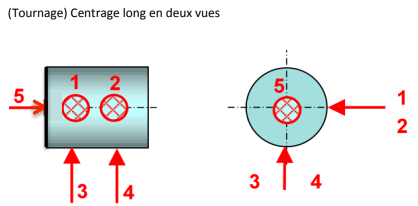
\includegraphics[width=0.6\textwidth]{Images/C11.PNG} % Include the figure image

	\label{fig:placeholder} % Unique label used for referencing the figure in-text
\end{figure}




\subsubsection{Centrage Court}
Nous ferons un centrage court quand la pièce ne permet pas de s'appuyer sur le long de la pièce. On construira contact plan.
\begin{itemize}
    \item Liaison linéaire annulaire (2 normales de repérage : 4 et 5)
    \item Liaison appui plan (3 normales de repérage : 1, 2 et 3)
\end{itemize}
 \begin{figure}[H] % Use [H] to suppress floating and place the figure/table exactly where it is specified in the text
	\centering % Horizontally center the figure on the page
	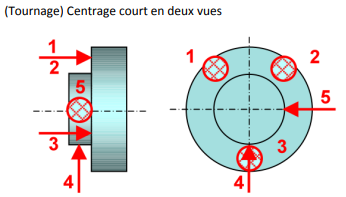
\includegraphics[width=0.6\textwidth]{Images/C22.PNG} % Include the figure image

	\label{fig:placeholder} % Unique label used for referencing the figure in-text
\end{figure}




%----------------------------------------------------------------------------------------
%	PRESENTING INFORMATION/RESULTS EXAMPLES CHAPTER
%----------------------------------------------------------------------------------------

\chapterimage{Images/BB1.jpg} % Chapter heading image
\chapterspaceabove{6.25cm} % Whitespace from the top of the page to the chapter title on chapter pages
\chapterspacebelow{7.5cm} % Amount of vertical whitespace from the top margin to the start of the text on chapter pages

%------------------------------------------------

\chapter{Lecture de l'information}

\textbf{Pour ce chapitre, nous ferons toujours référence au dessin de définition de l'annexe.}

\section{Norme ISO 2768mk}
Un côte possède TOUJOURS un intervalle de tolérance. Cependant, pour avoir une meilleure lisibilité, certaine tolérance ne sont pas directement présente sur le dessin de définition. Dans ce cas, il faudra vous référer aux indications du dessin de définition. Le plus souvent, vous aurez la norme ISO 2768mk. Il faudra alors regarder la ligne correspondant pour trouver l'intervalle de tolérance.
 \begin{figure}[H] % Use [H] to suppress floating and place the figure/table exactly where it is specified in the text
	\centering % Horizontally center the figure on the page
	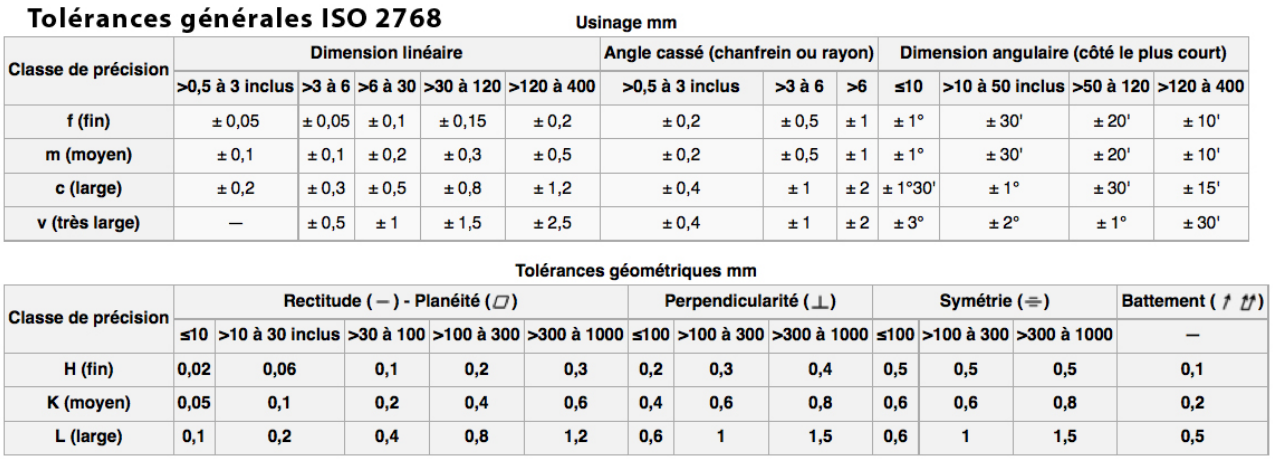
\includegraphics[width=1\textwidth]{Images/T13.PNG} % Include the figure image

	\label{fig:placeholder} % Unique label used for referencing the figure in-text
\end{figure}



\section{Ajustement}
Les ajustements sont indiqués par des lettres sur le dessin de définition. Par exemple $30\varnothing$H7. La tolérance de cet ajustement est alors à chercher sur internet ou dans vos cours.
 \begin{figure}[H] % Use [H] to suppress floating and place the figure/table exactly where it is specified in the text
	\centering % Horizontally center the figure on the page
	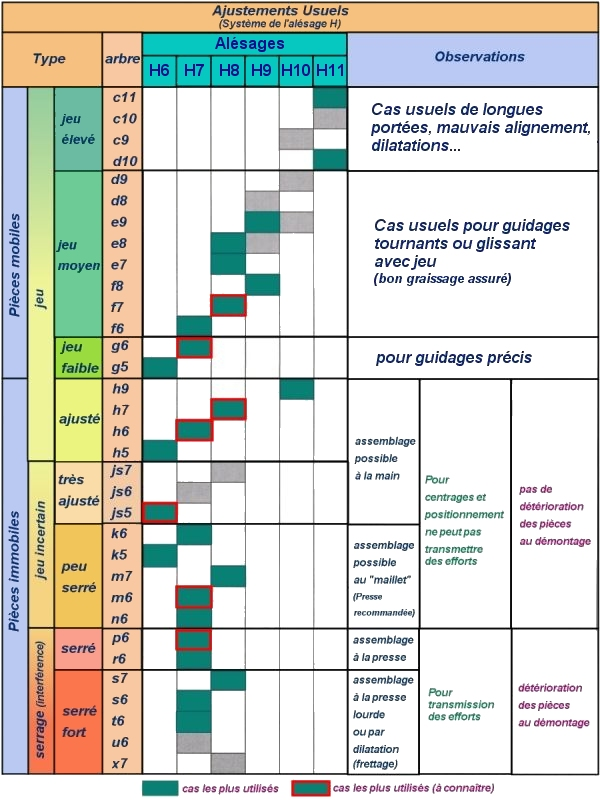
\includegraphics[width=1\textwidth]{Images/AA11.jpg} % Include the figure image

	\label{fig:placeholder} % Unique label used for referencing the figure in-text
\end{figure}
Pour exemple, $30\varnothing$H7 est écrit avec un "H" majuscule, c'est donc un \textbf{alésage} (c'est la pièce extérieur). Alors que $34\varnothing$f7 possède un "f" minuscule, c'est donc un \textbf{arbre} (c'est la pièce intérieur).


\section{Ébauche et finition}
Pour savoir si vous devez faire seulement une finition, ou une ébauche + une demi finition + une finition, vous utiliserez le tableau ci-dessous, trouvable aussi sur internet.
 \begin{figure}[H] % Use [H] to suppress floating and place the figure/table exactly where it is specified in the text
	\centering % Horizontally center the figure on the page
	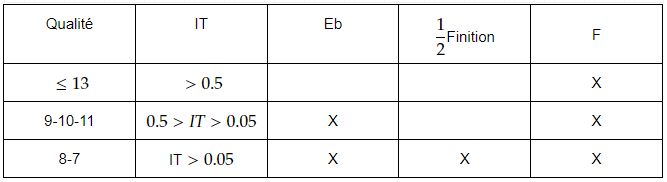
\includegraphics[width=1\textwidth]{Images/Ebauche.PNG} % Include the figure image

	\label{fig:placeholder} % Unique label used for referencing the figure in-text
\end{figure}

Pour l'état de surface, le tableau suivant :
 \begin{figure}[H] % Use [H] to suppress floating and place the figure/table exactly where it is specified in the text
	\centering % Horizontally center the figure on the page
	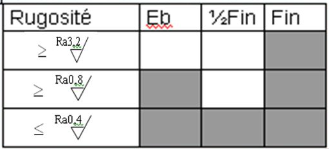
\includegraphics[width=0.6\textwidth]{Images/Ebauche2.PNG} % Include the figure image

	\label{fig:placeholder} % Unique label used for referencing the figure in-text
\end{figure}


\newpage
\section{ANNEXE}
 \begin{figure}[H] % Use [H] to suppress floating and place the figure/table exactly where it is specified in the text
	\centering % Horizontally center the figure on the page
	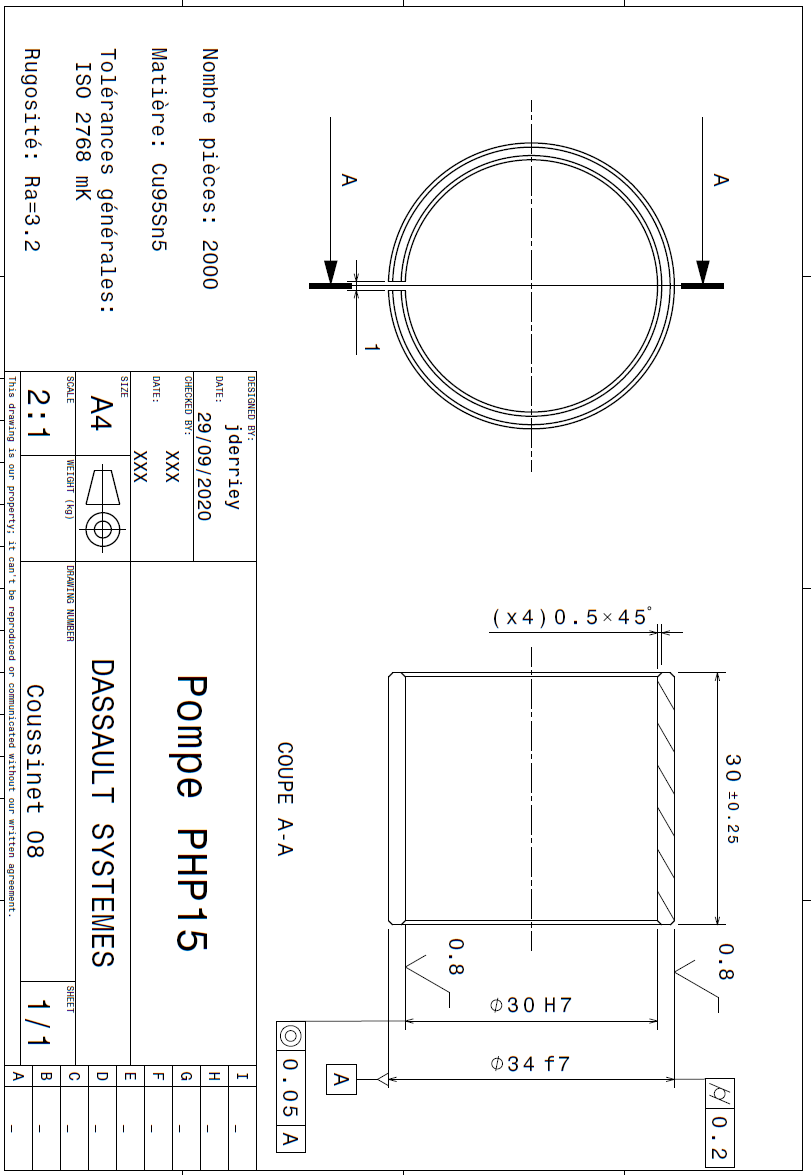
\includegraphics[width=1\textwidth]{Images/D11.PNG} % Include the figure image

	\label{fig:placeholder} % Unique label used for referencing the figure in-text
\end{figure}

\end{document}


